\documentclass[10pt,a4paper]{jarticle}

\usepackage[top=25truemm,bottom=25truemm,left=20truemm,right=20truemm]{geometry}
\usepackage[dvipdfmx]{graphicx}
\usepackage{amsmath}
\usepackage{float}
\usepackage{booktabs}
\usepackage{listings}
\usepackage{url}

\lstset{
  basicstyle={\small\ttfamily},
  breaklines=true,
  frame=single,
  tabsize=3,
  language=Python,
  columns=fullflexible,
  keepspaces=true
}

\begin{document}

%==================================================
% 表紙
%==================================================
\begin{titlepage}
  \thispagestyle{empty}

  % 上部の授業名・レポート種別
  \begin{center}
    {\Large ビッグデータ特論\par}
    \vspace{0.4em}
    {\Large 期末レポート\par}

    \vspace{2.5em}

    % レポートタイトル
    {\fontsize{28pt}{42pt}\selectfont
      自己注意機構における\par
      \vspace{0.5em}
      知識の形成と利用\par
    }
  \end{center}

  \vfill

  % 右下の提出者情報
  \begin{flushright}
    \begin{minipage}{0.43\textwidth}
      \renewcommand{\arraystretch}{1.35}
      \begin{tabular}{@{}ll@{}}
        選択カテゴリ &：カテゴリB \\
        トピック     &：自己注意機構 \\
                     & \\
        専攻         &：情報創成工学専攻 \\
        学年         &：1年 \\
        研究室名     &：大北研究室 \\
        学生番号     &：266E0017 \\
        氏名         &：大田重吉 \\
        提出年月日   &：2026年7月25日
      \end{tabular}
    \end{minipage}
  \end{flushright}

\end{titlepage}

%==================================================
% 本文
%==================================================

\section{はじめに}
自己注意機構とは、ChatGPTなどの大規模言語モデルや、多くの画像生成モデルを支えるTransformerという深層学習モデルの中心部品である。その自己注意機構が現代の様々なAIモデルの知識をどう形成し、どう利用しているのかを説明する。

\subsection{複数の要素から必要な情報を選ぶ問題}
自己注意機構が対象としている問題は、「複数の要素を入力として受け取り、各要素がほかの要素から必要な情報をどのように参照するかを決定する」というものである。例として、「少年がリンゴを食べた。それは赤かった。」という文章では、「それ」だけでは何を指すか分からないが、前の「少年」「リンゴ」「食べた」を比べれば、「赤かった」と自然につながるのは「リンゴ」だと判断できる。こういった判断のための情報の参照方法を自己注意機構が担当する。

\subsection{自己注意機構が行うこと}
自己注意機構の簡略化したアルゴリズムを以下に示す。またこれらの仕組みは実際には行列演算で行われるので、行列積の意味について次の章で解説する。

\begin{lstlisting}[caption=自己注意機構の簡略アルゴリズム,label=lst:simple_attention]
query = make_query(inputs)
key = make_key(inputs)
value = make_value(inputs)
reference_table = compare(query, key)
outputs = collect(value, reference_table)
\end{lstlisting}


\section{行列積の意味}
ここでは自己注意機構を実現するための前提知識である行列積について解説する。

\subsection{要素はベクトルで表される}
入力される複数の要素はそれぞれベクトルとしてあらわされ、入力全体はそれらのベクトルが並んだ行列としてあらわされる。
\begin{figure}[H]
  \centering
  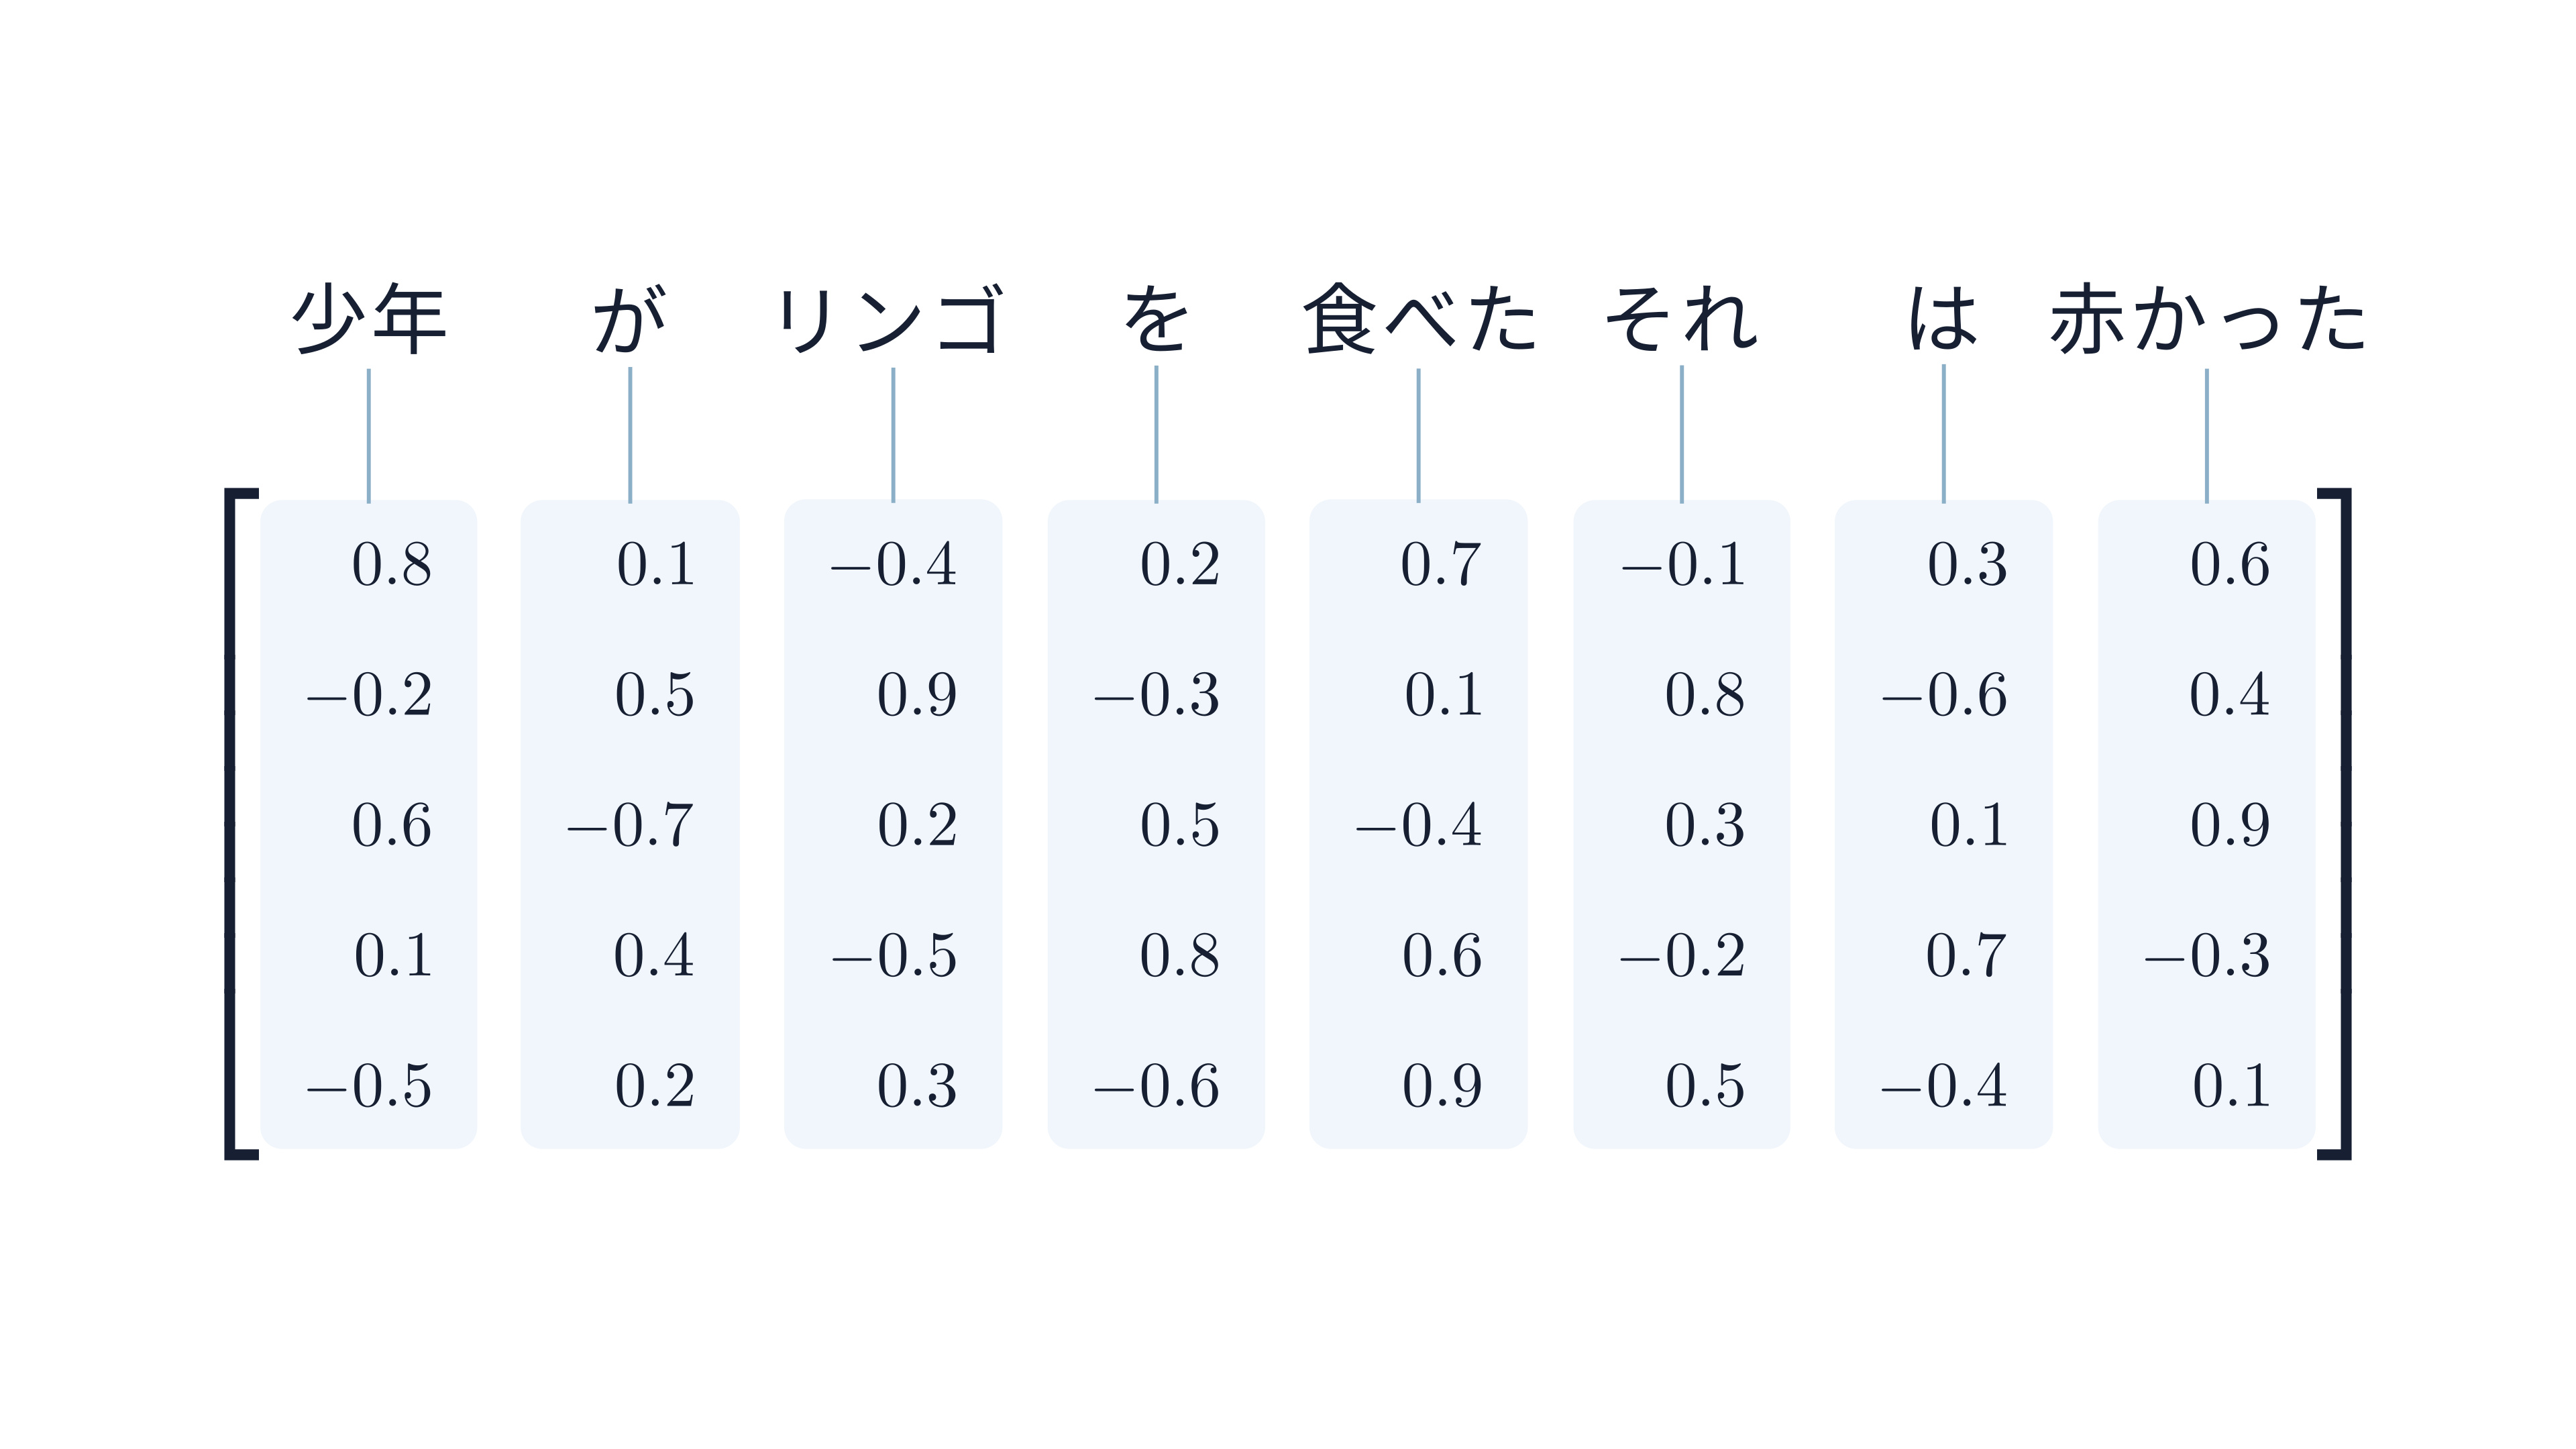
\includegraphics[width=\linewidth]{figures/fig01_tokens_to_vectors.jpg}
  \caption{入力文のベクトル表現}
  \label{fig:tokens-to-vectors}
\end{figure}

\subsection{内積は「質問への反応」}
内積はその二点の成分の近さを示す。ある要素を表すベクトルと、質問的な意味合いを持つベクトルの内積を考えると、これはある種の質問応答のように解釈することができる。（もちろん実際には具体的な質問ではなく幾何学上のパターンマッチングである。）
\begin{figure}[H]
  \centering
  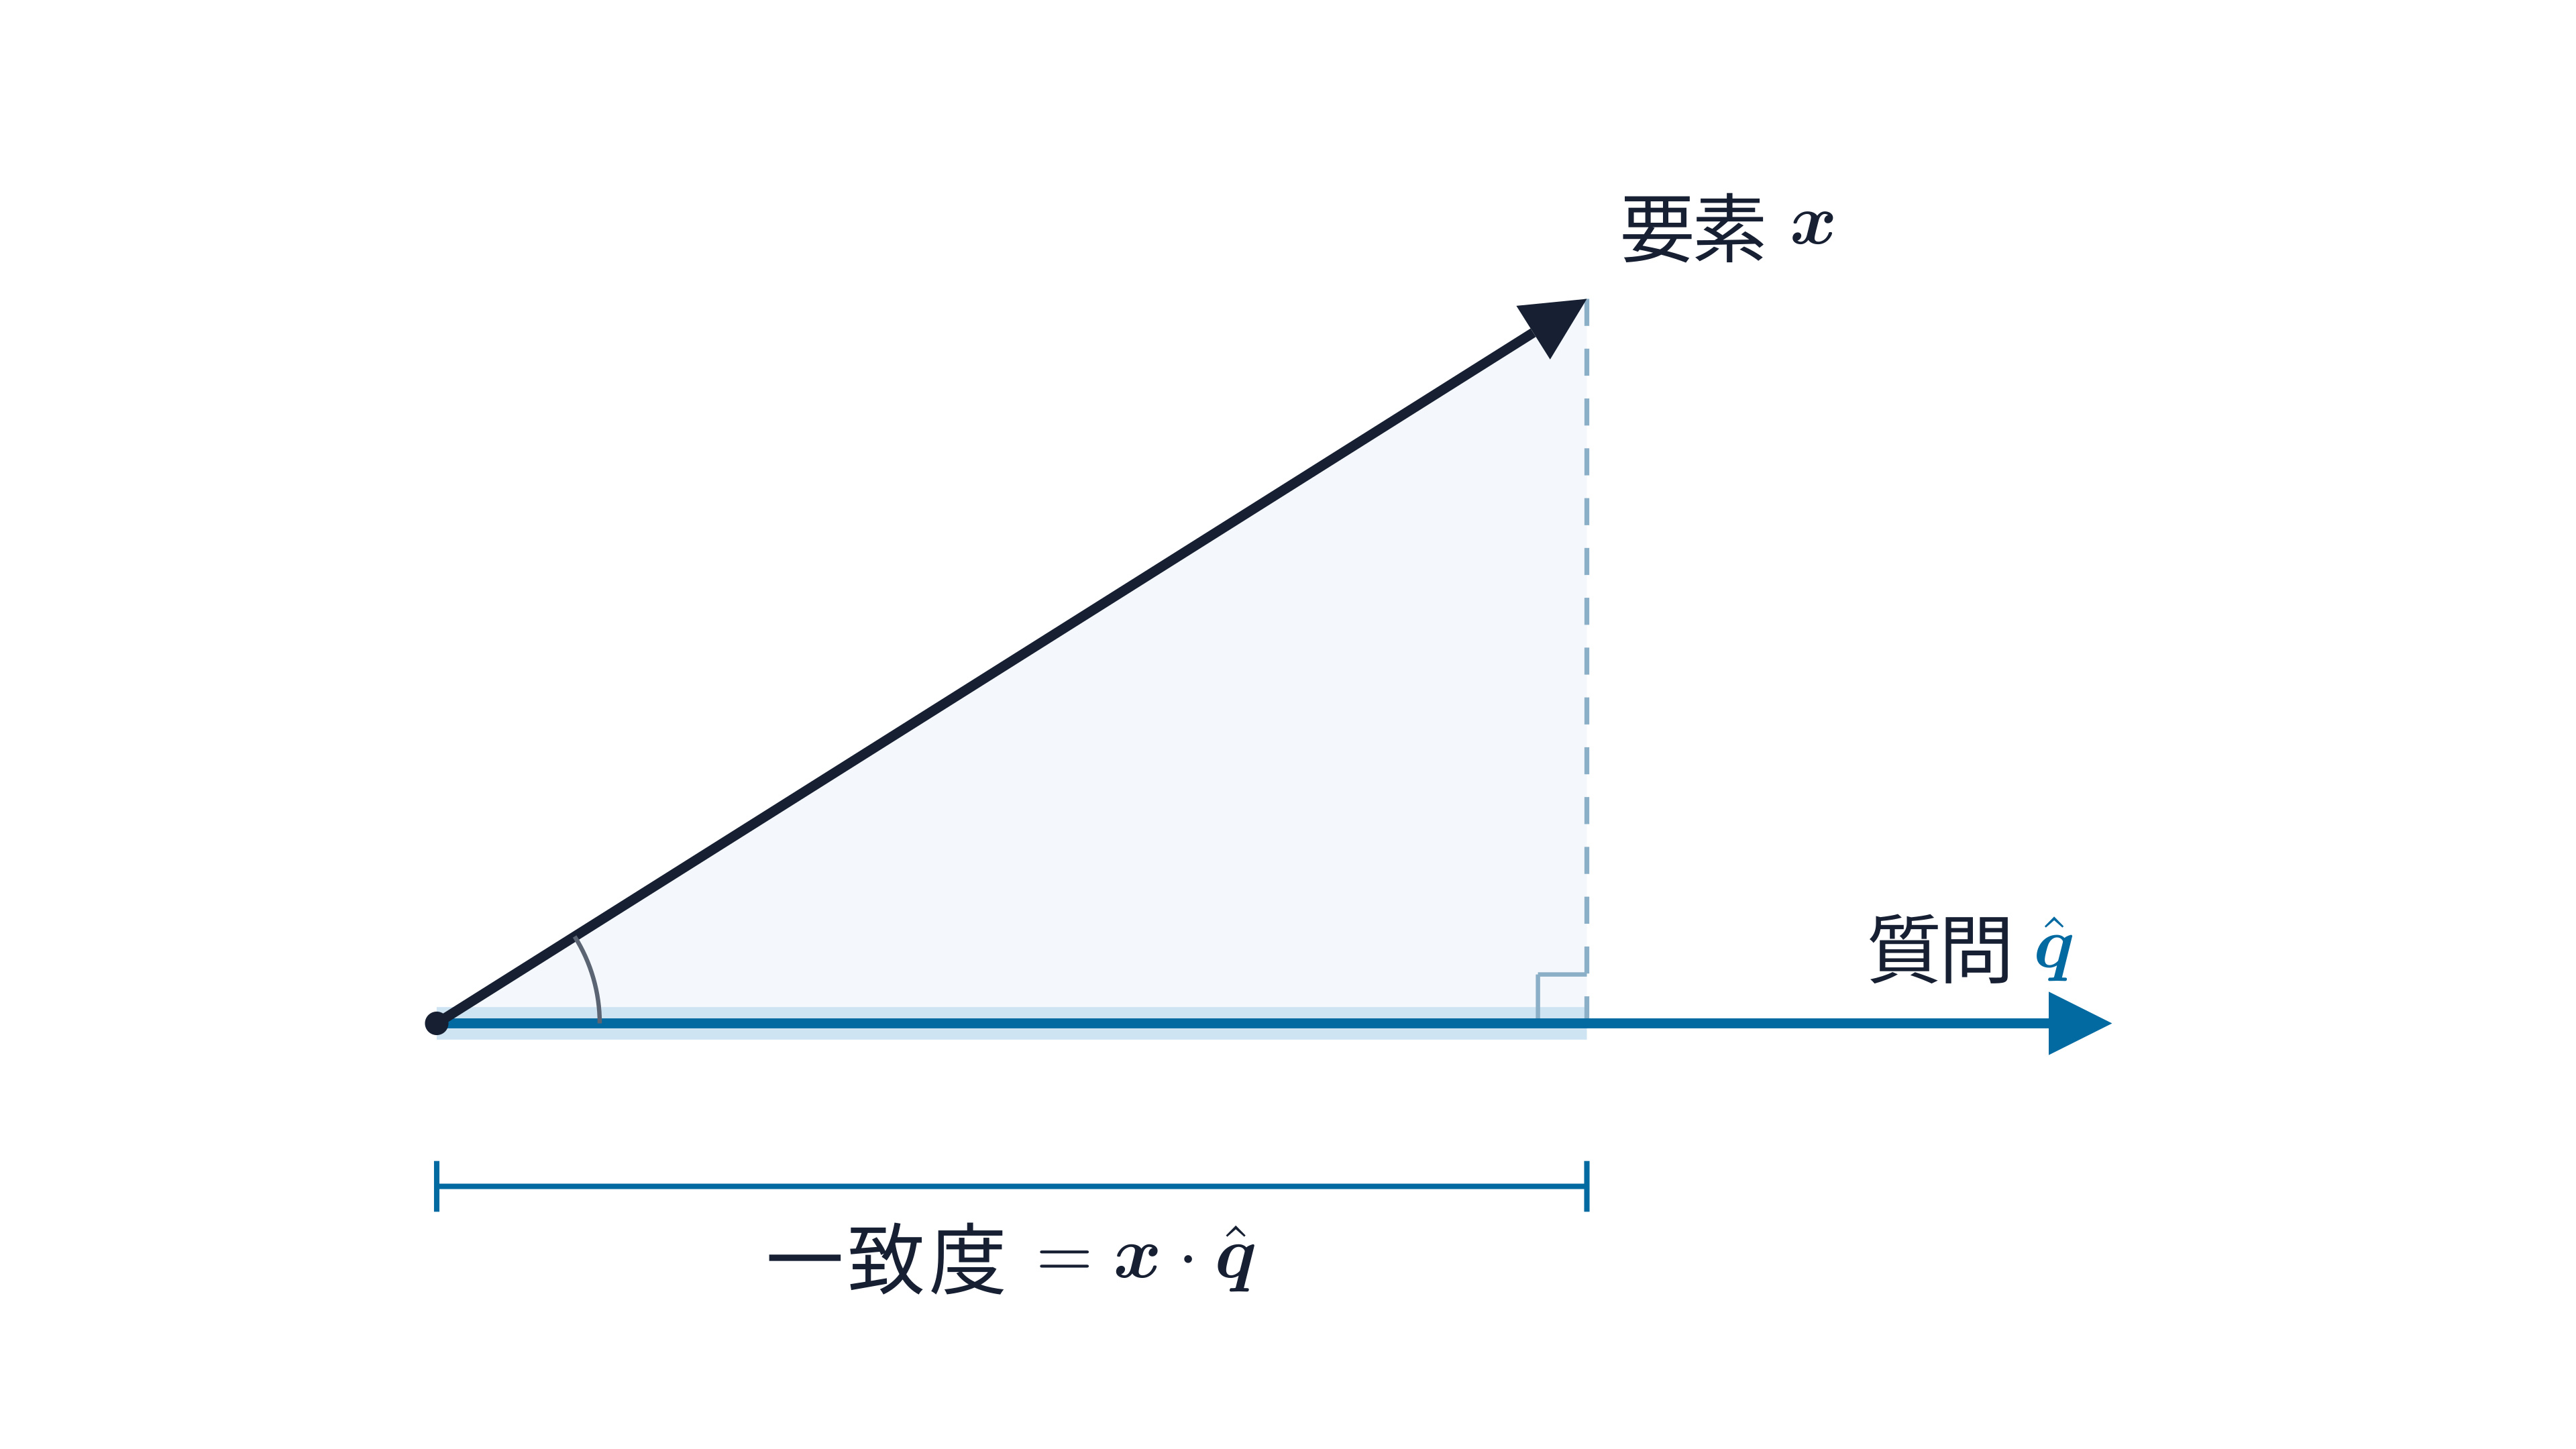
\includegraphics[width=\linewidth]{figures/fig02_inner_product_projection.jpg}
  \caption{質問方向への射影}
  \label{fig:inner-product-projection}
\end{figure}

\subsection{行列積は「全組み合わせの内積を並べた表」}
要素ベクトル群によって構成された行列と質問ベクトル群によって構成された行列の行列積は、各要素ベクトルに各質問ベクトルの内積を取った値を表のように並べたものになる。
\begin{figure}[H]
  \centering
  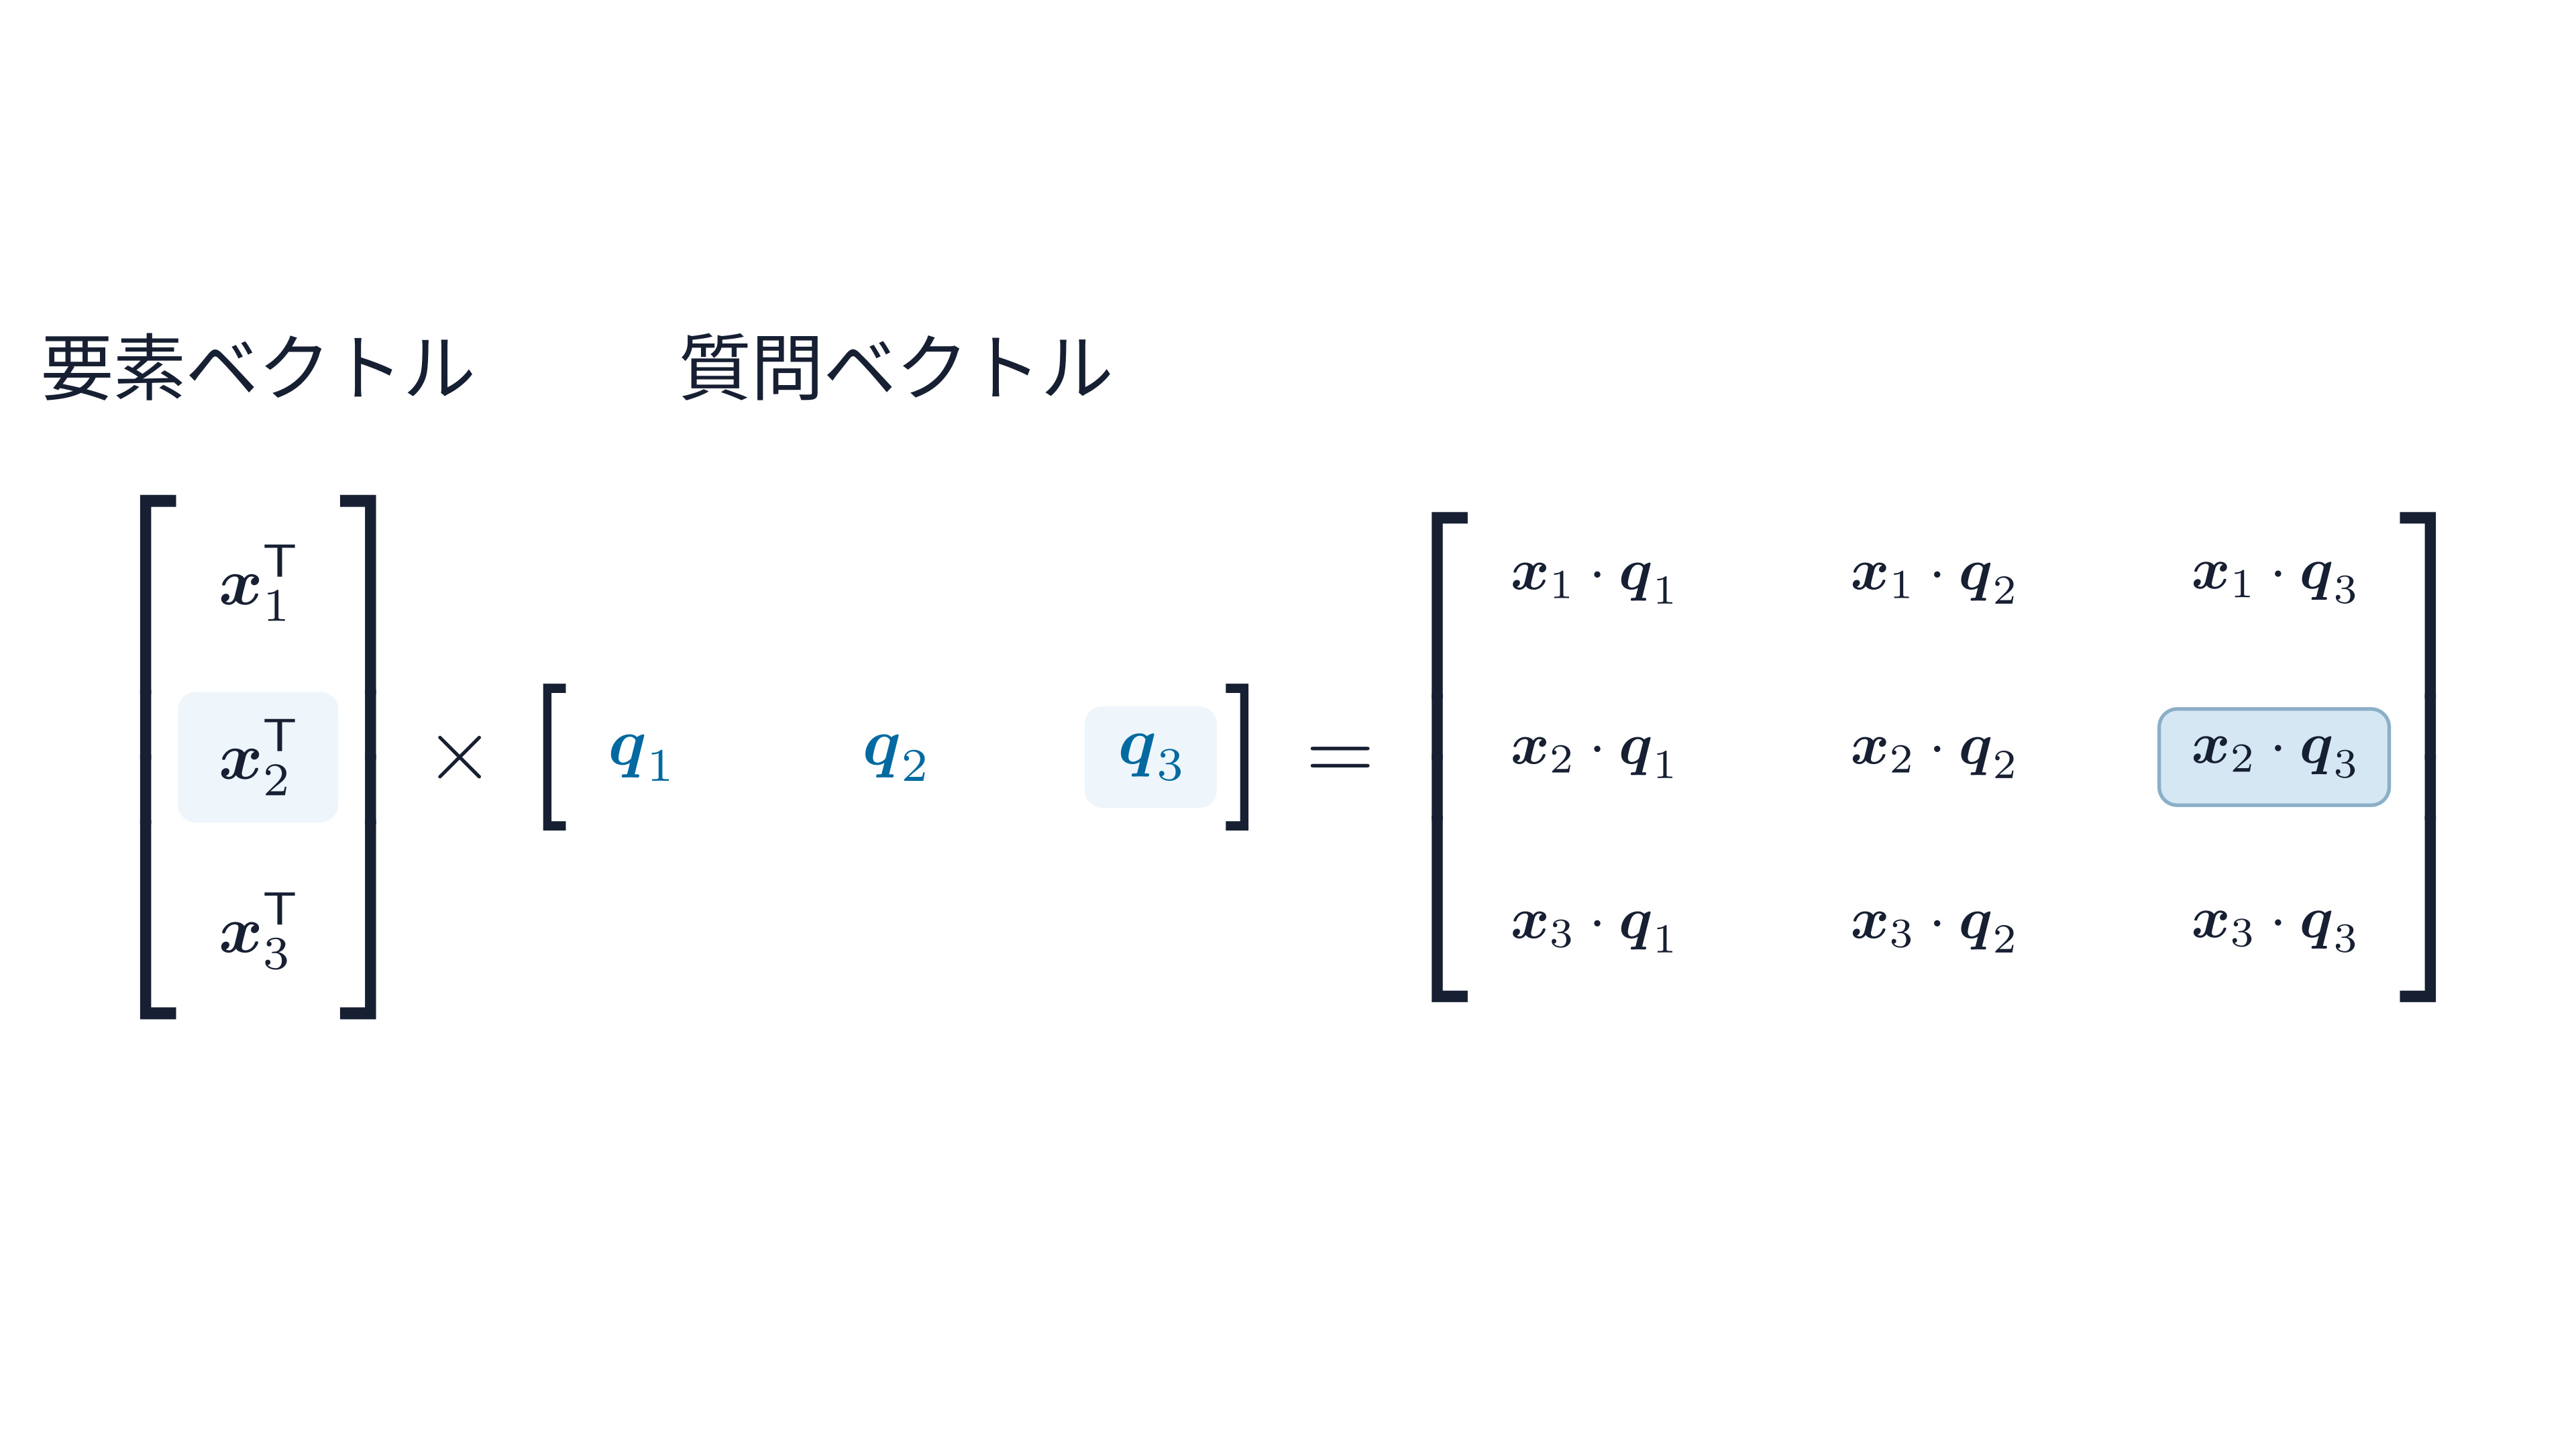
\includegraphics[width=\linewidth]{figures/fig03_all_pairwise_inner_products.jpg}
  \caption{行列積で得られる内積表}
  \label{fig:all-pairwise-inner-products}
\end{figure}


\section{自己注意機構のアルゴリズム}
ここではより詳細な自己注意機構のアルゴリズムについて解説する。

\subsection{自己注意機構の持ち物}
Query、Key、Valueを作るための三つの質問行列を持つ。これらの行列は入力に対して、「ほかの入力に何を問いかけるか」「ほかの入力からの問いにどう答えるか」「どのような情報を伝えるか」をそれぞれ複数の観点から問う。
\begin{figure}[H]
  \centering
  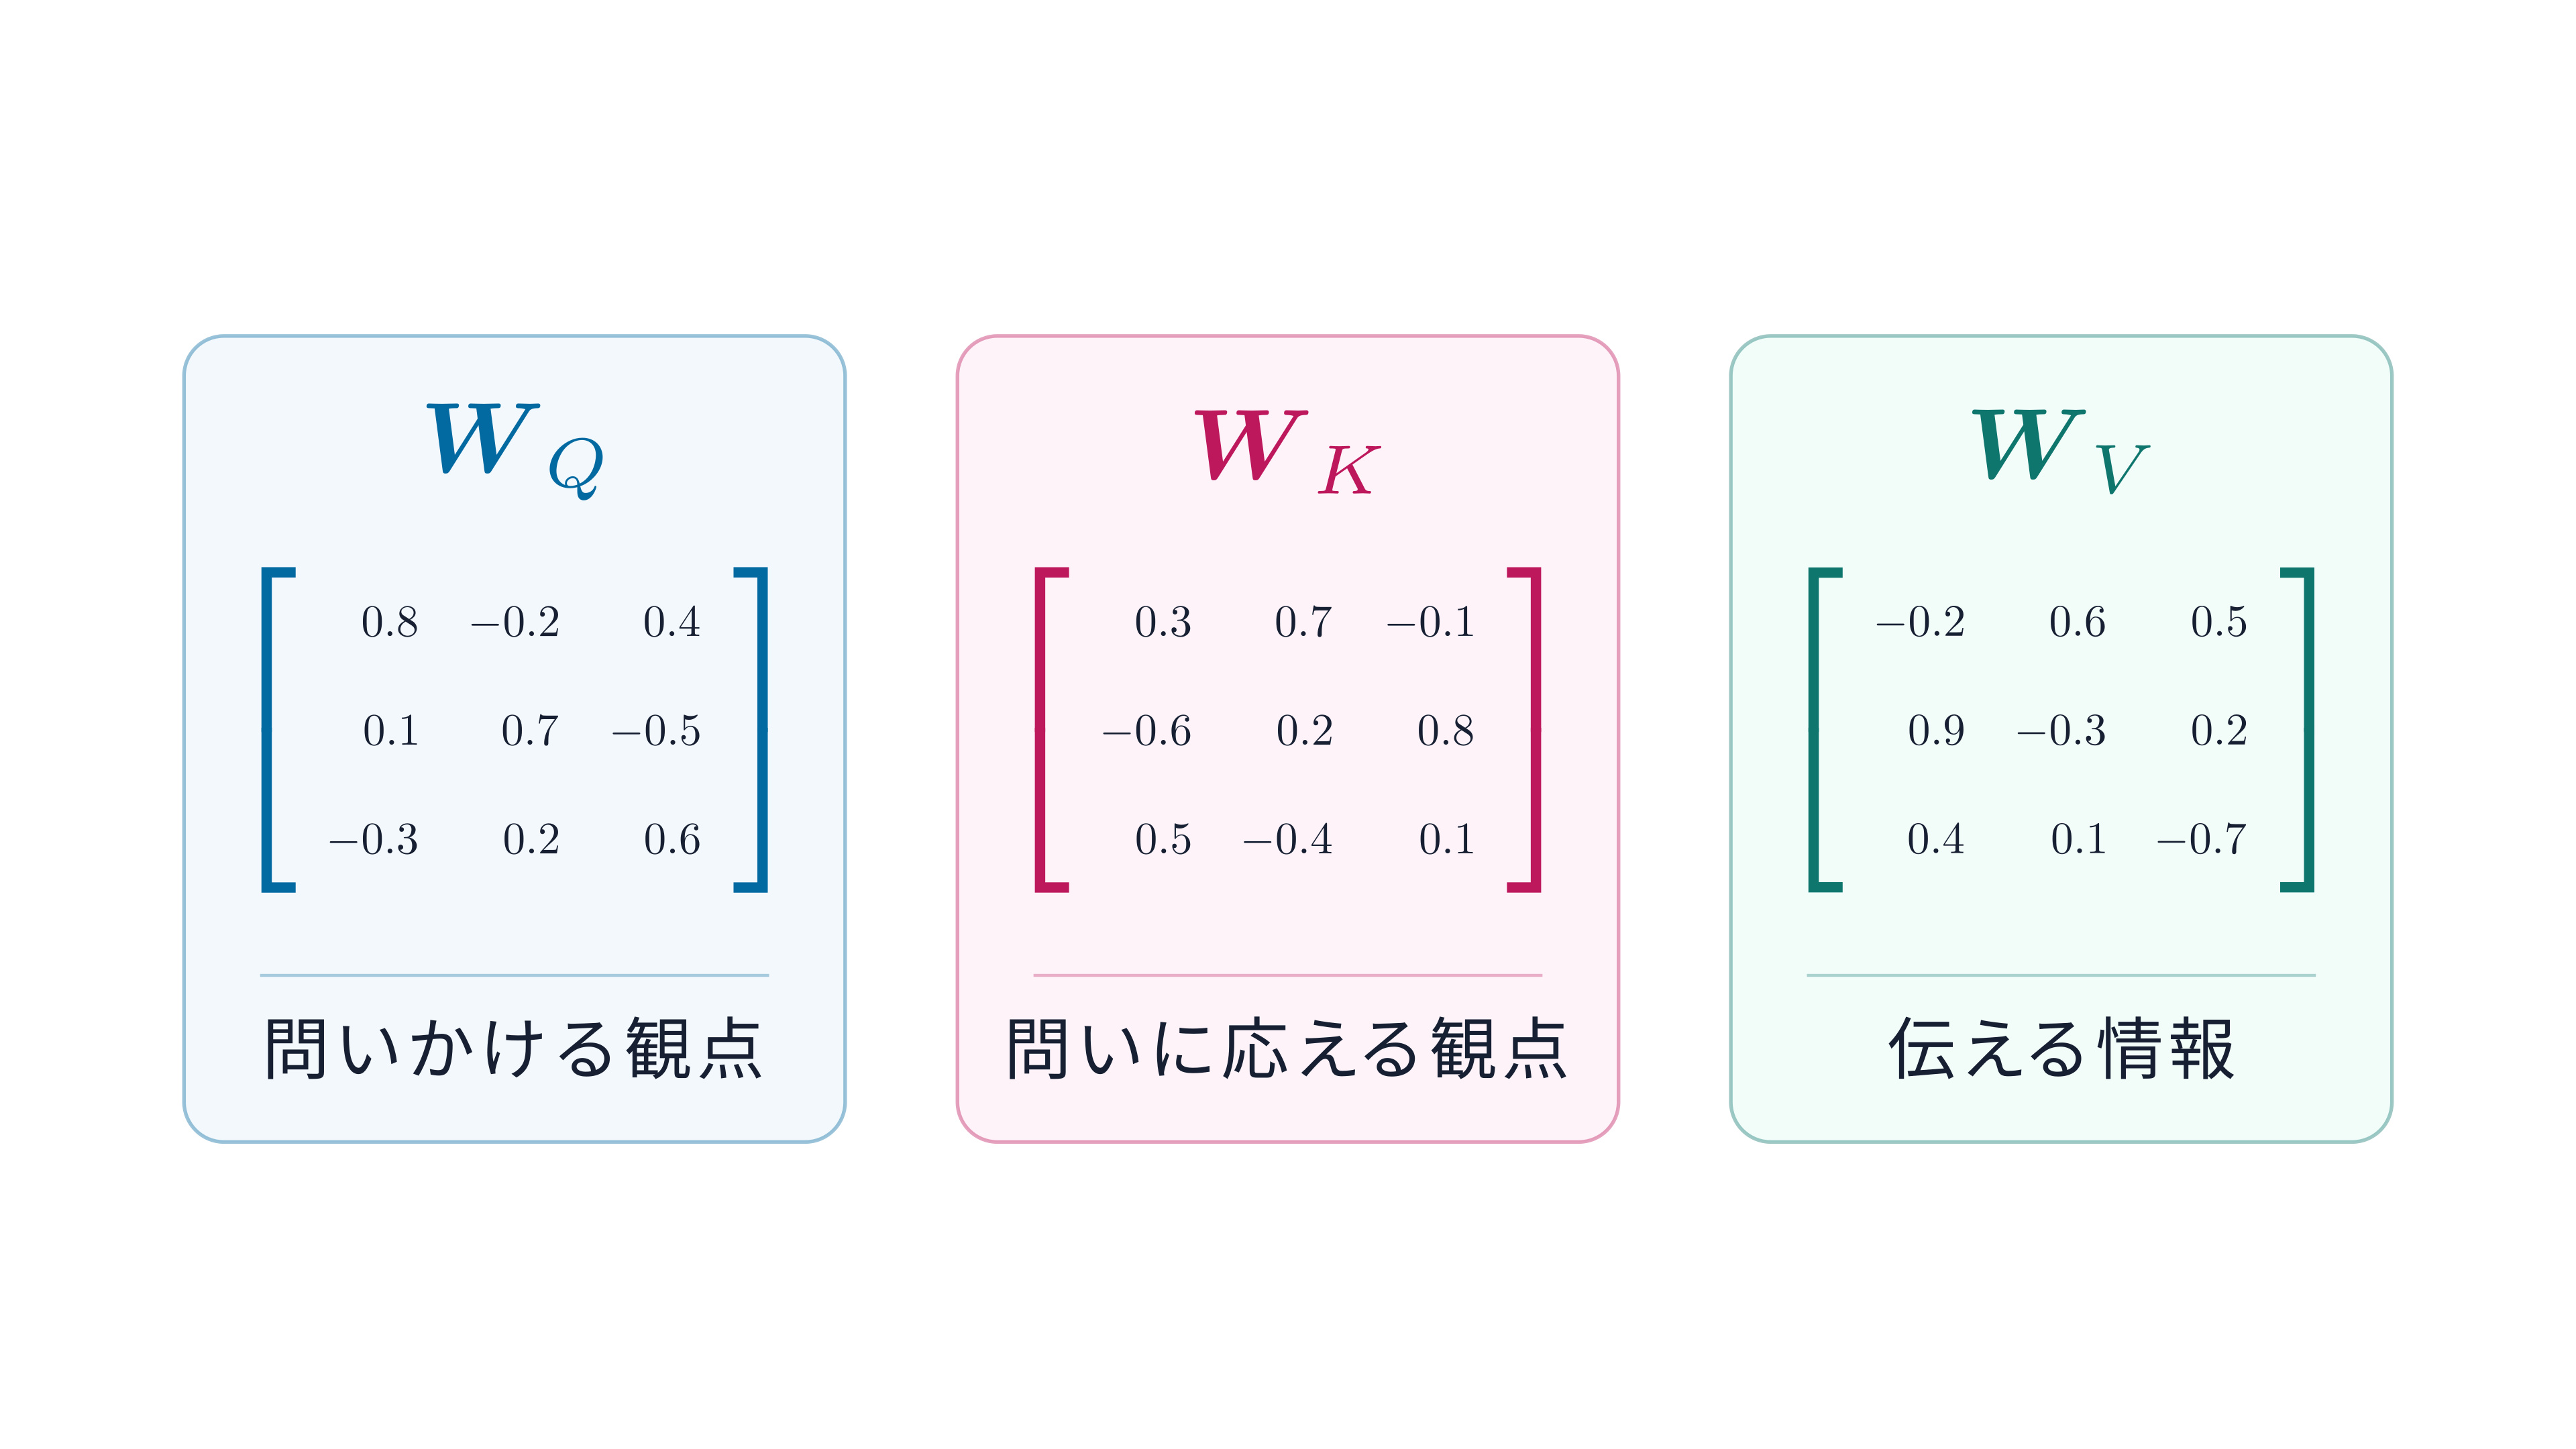
\includegraphics[width=\linewidth]{figures/fig04_self_attention_parameters.jpg}
  \caption{三つの重み行列}
  \label{fig:self-attention-parameters}
\end{figure}

\subsection{入力からQuery、Key、Valueを作成}
入力行列と各質問行列の行列積を計算することでQuery・Key・Valueを作成する。入力に対して、Queryは「ほかの入力に何を問いかけるか」を、Keyは「ほかの入力からの問いにどう答えるか」をValueは「どのような情報を伝えるか」を表す。
\begin{figure}[H]
  \centering
  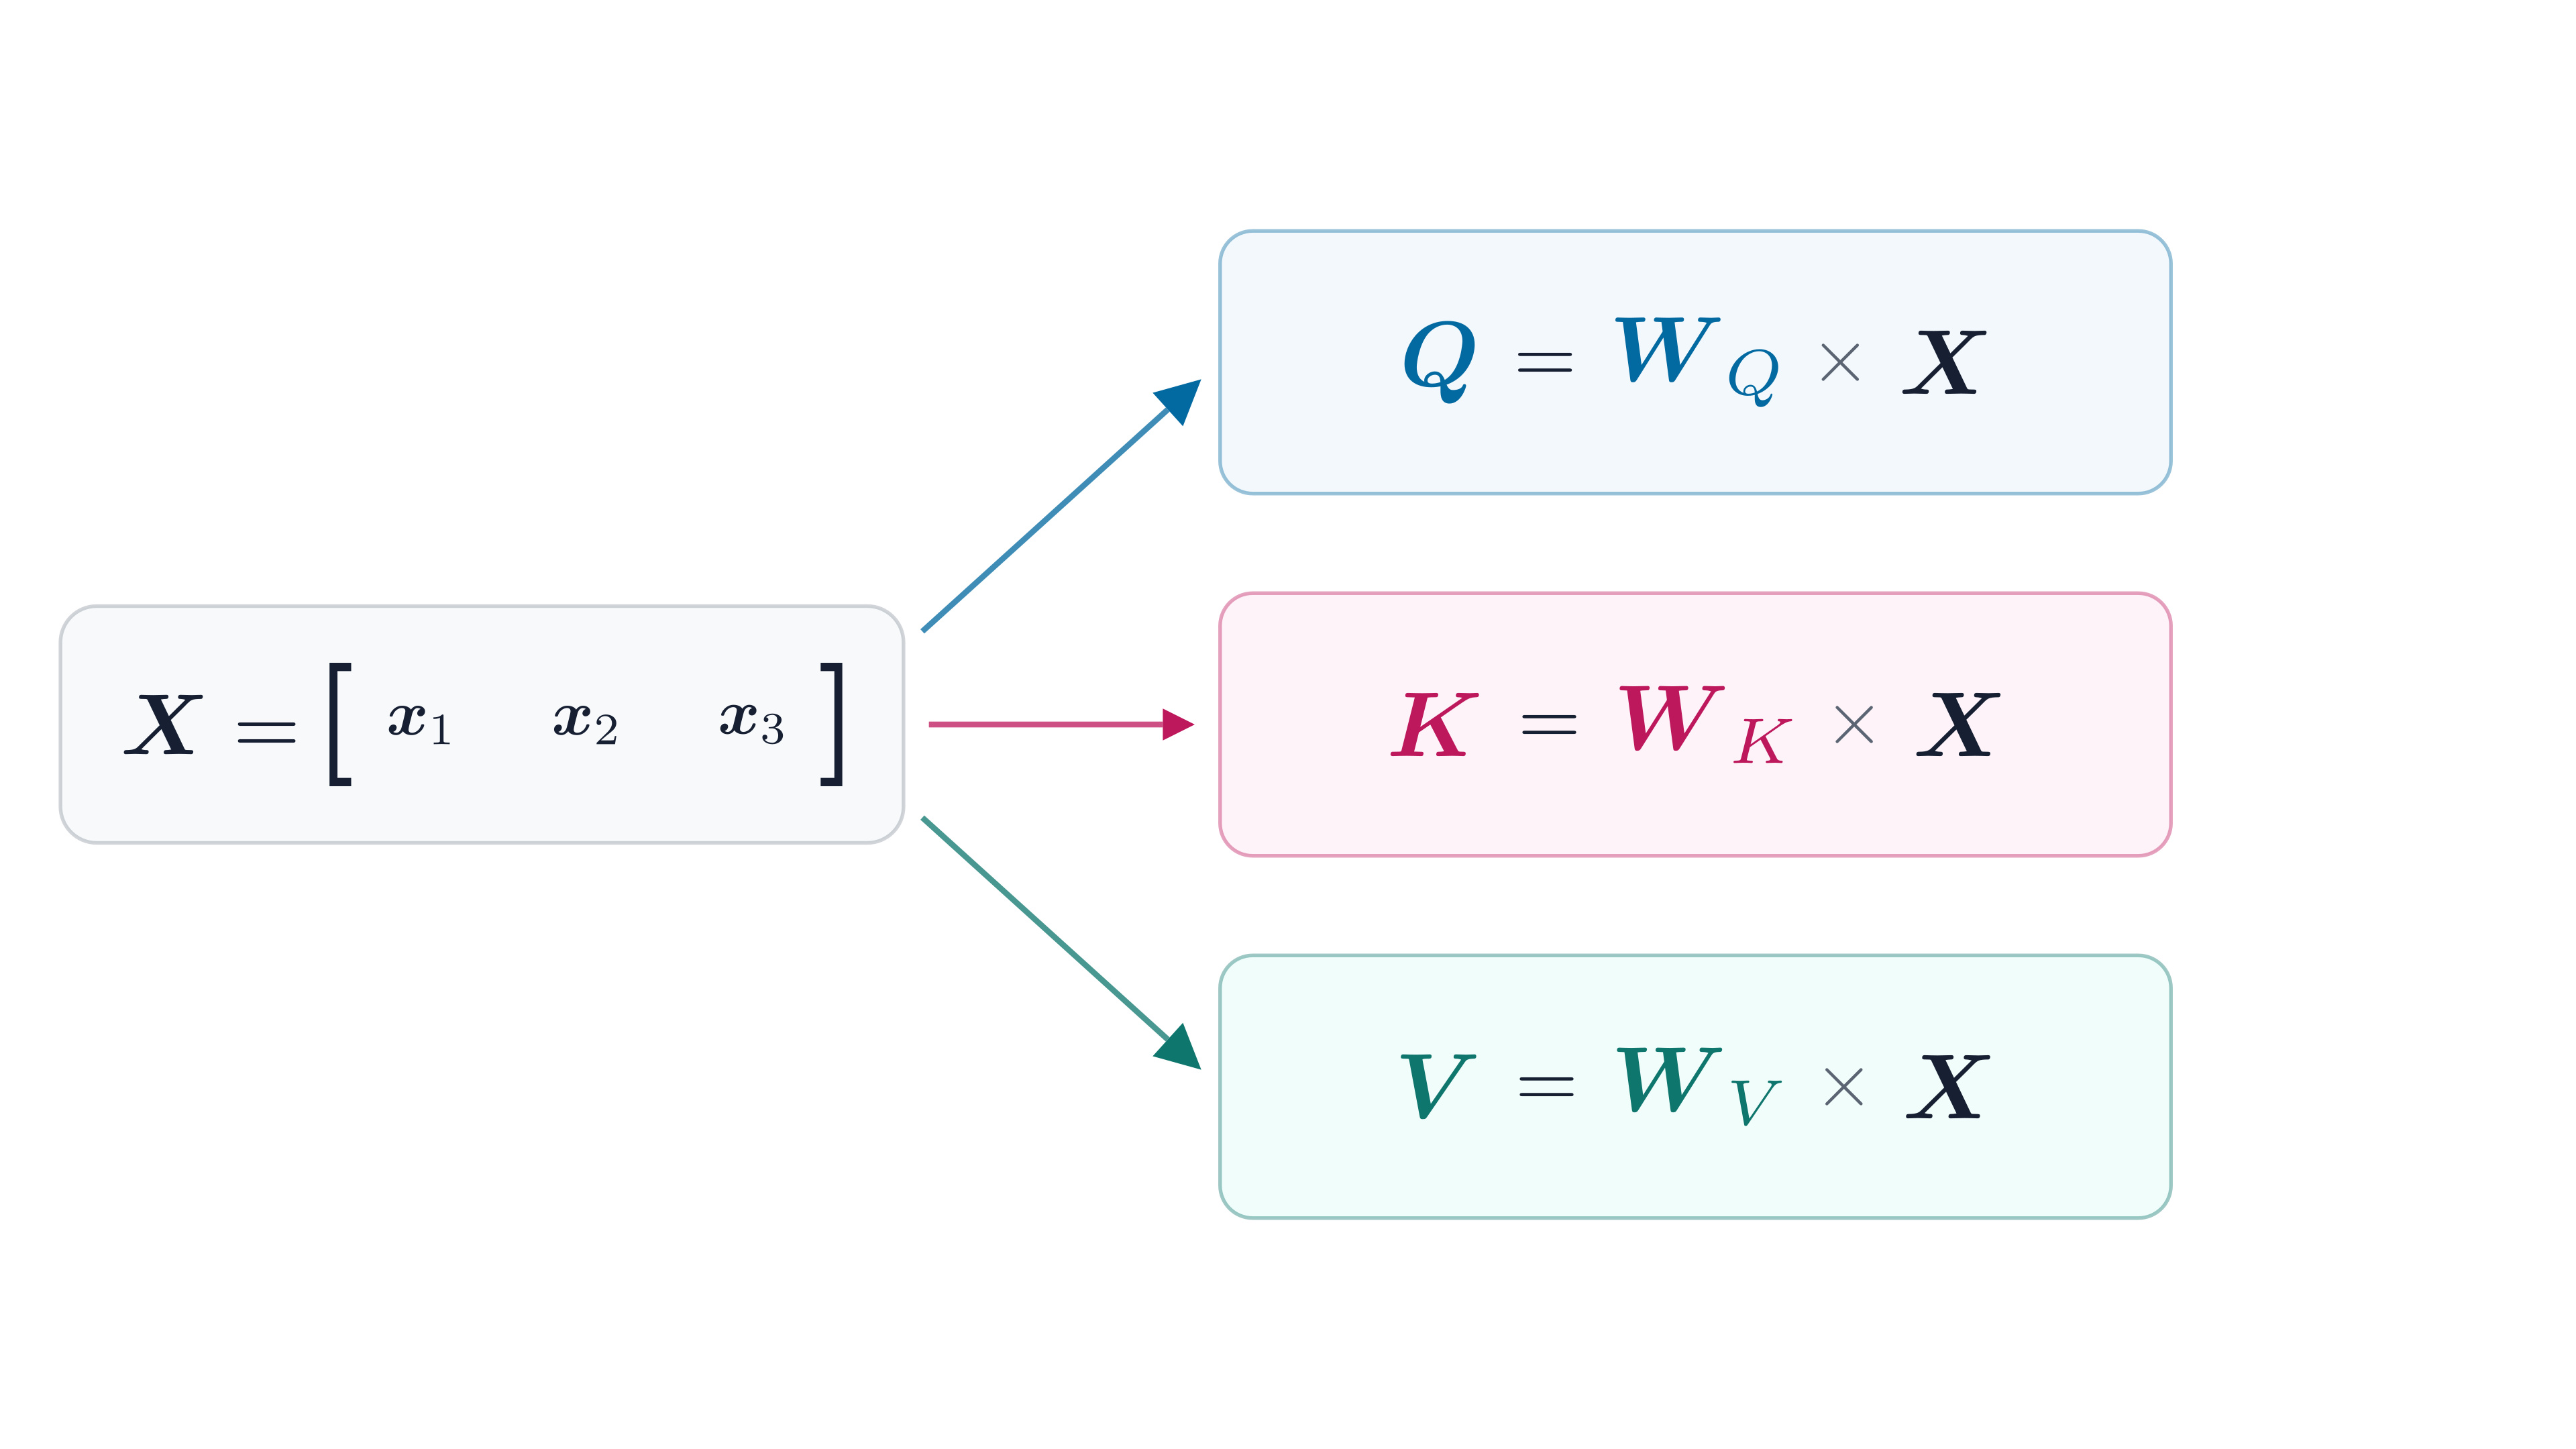
\includegraphics[width=\linewidth]{figures/fig05_create_query_key_value.jpg}
  \caption{入力から三つの表現への変換}
  \label{fig:create-query-key-value}
\end{figure}

\subsection{QueryとKeyの行列積で全要素の重み対応表を作成}
QueryとKeyの行列積を計算し、各入力の問いと、すべての入力の答えがどの程度一致するかを求める。これにより、各入力がほかの入力をどれだけ参照すべきかを表す重み対応表を作成する。
\begin{figure}[H]
  \centering
  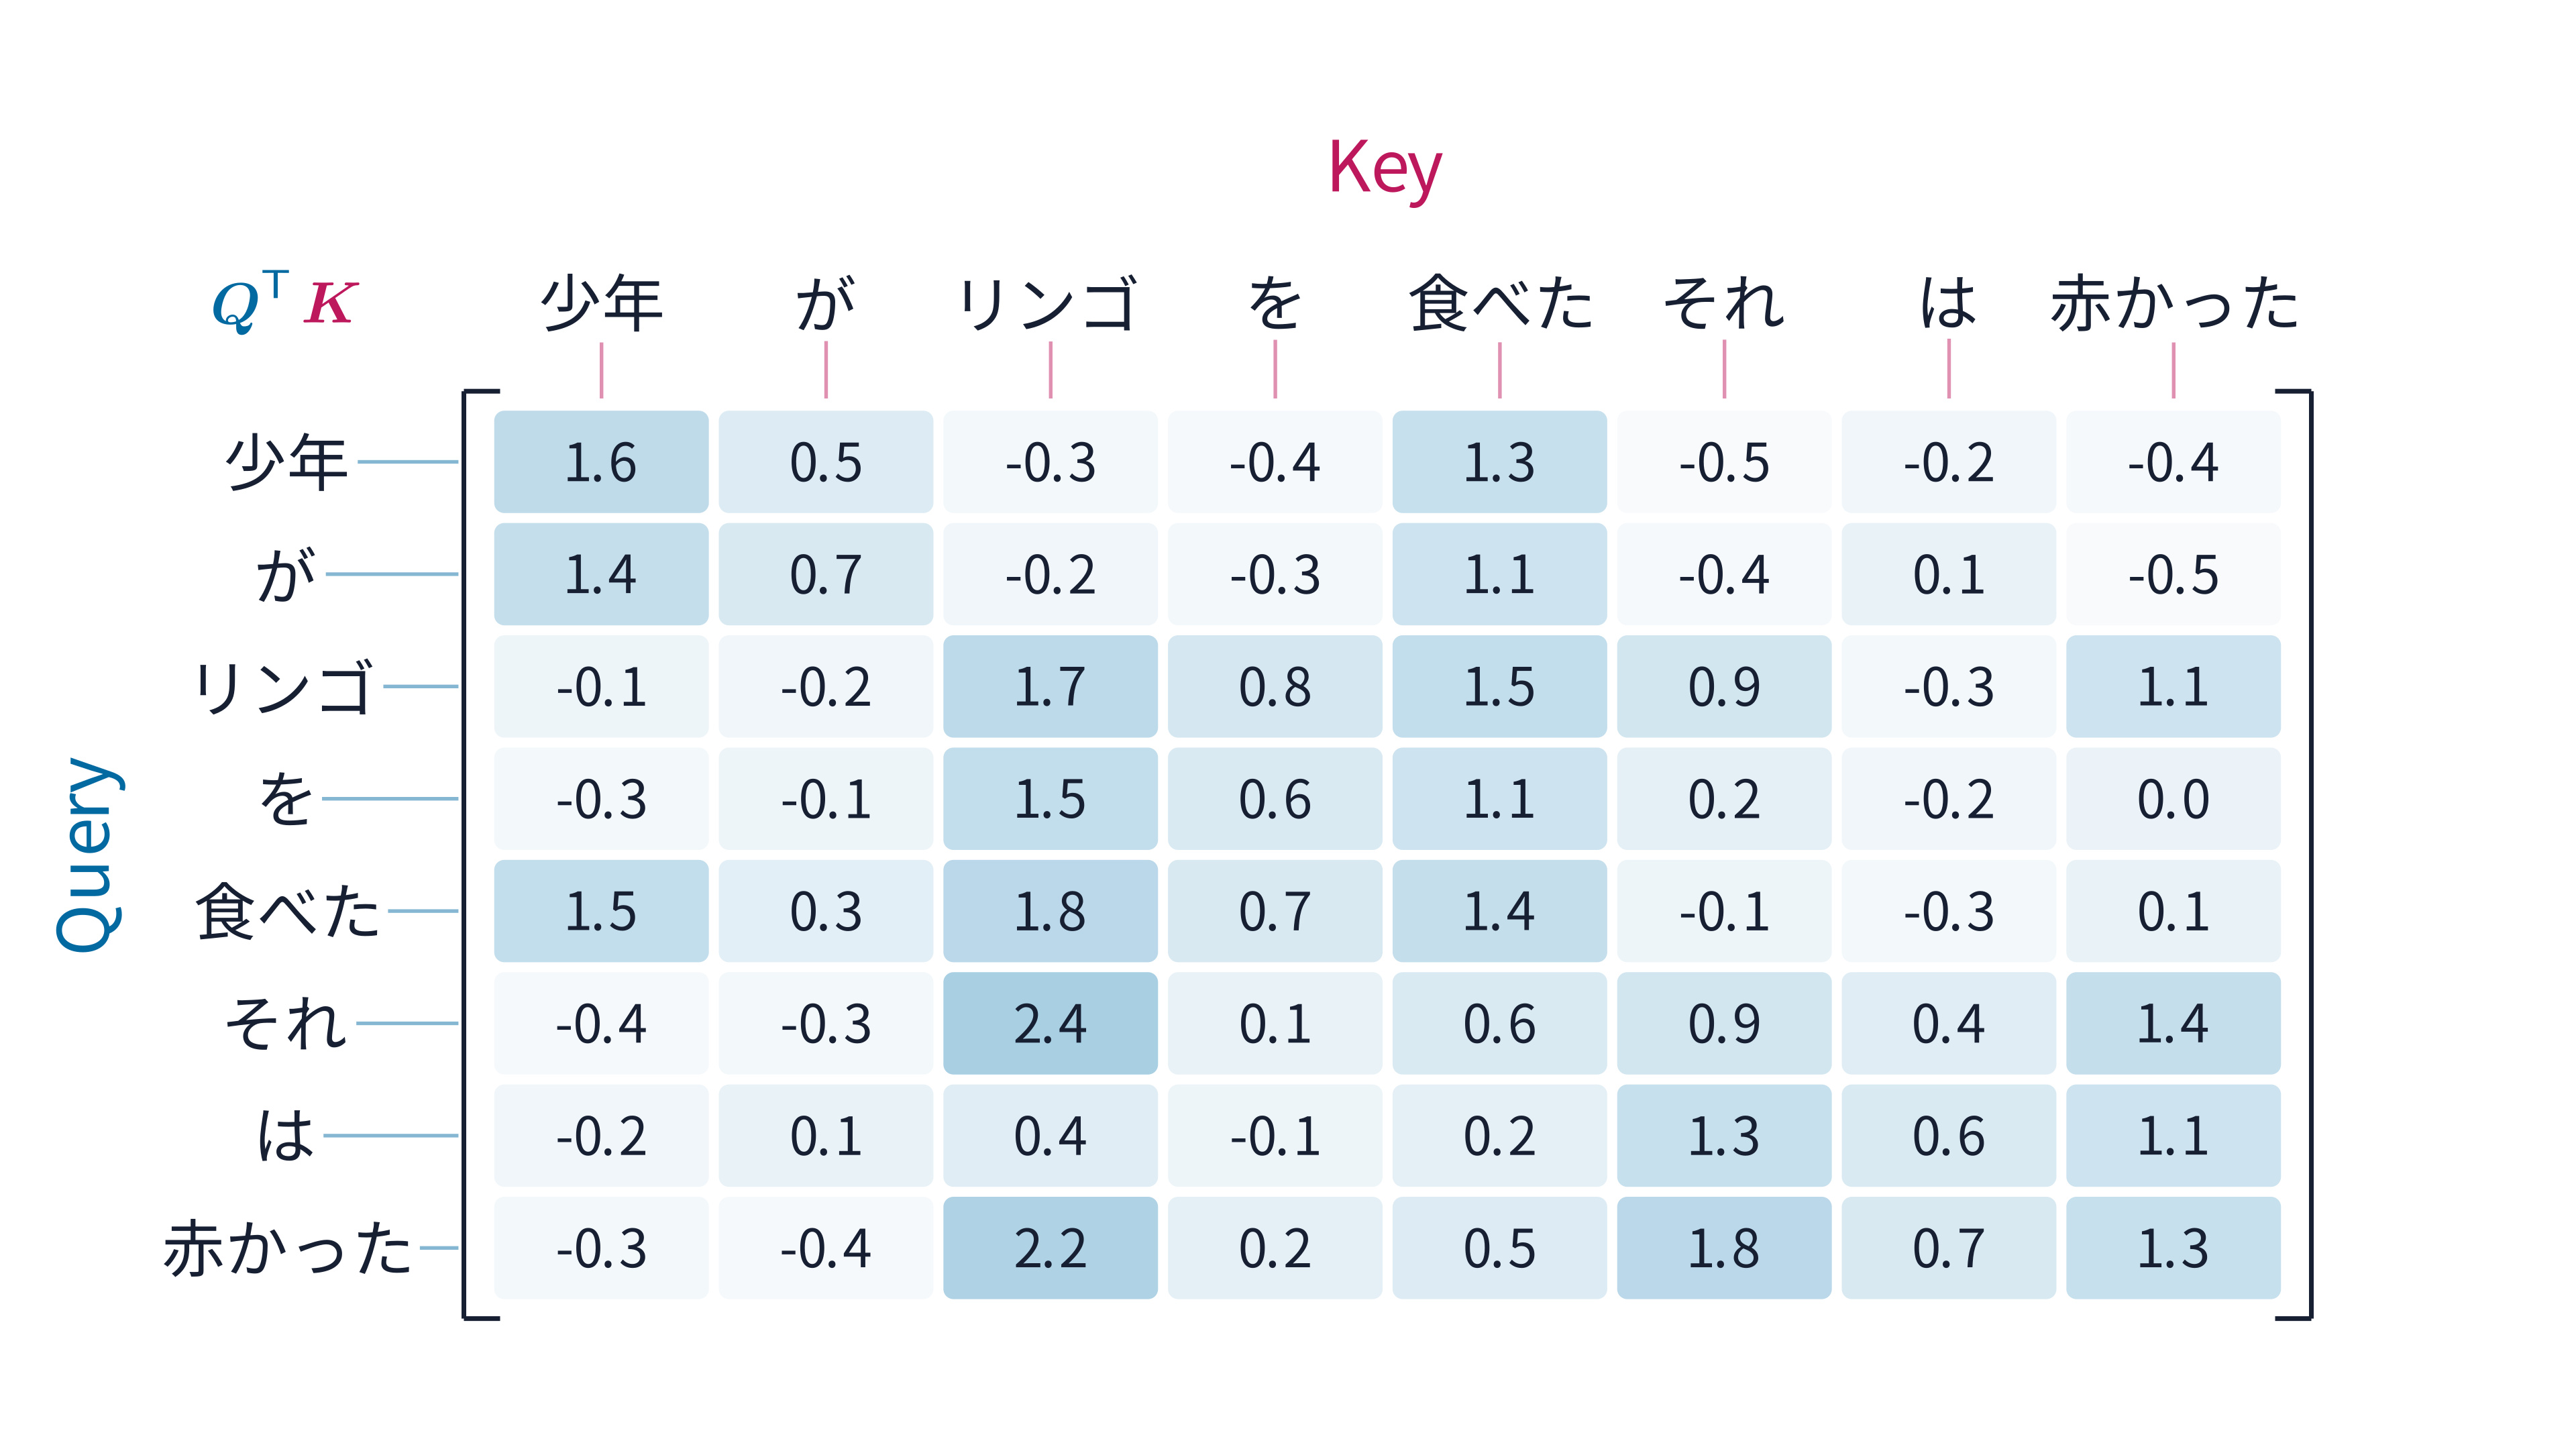
\includegraphics[width=\linewidth]{figures/fig06_query_key_score_table.jpg}
  \caption{各トークン間の一致度}
  \label{fig:query-key-score-table}
\end{figure}

\subsection{重みを参照割合に変換}
各重みにSoftmax関数を適用し、合計が1になる参照割合へ変換する。一致度が高い入力ほど、大きな割合で参照される。
\begin{figure}[H]
  \centering
  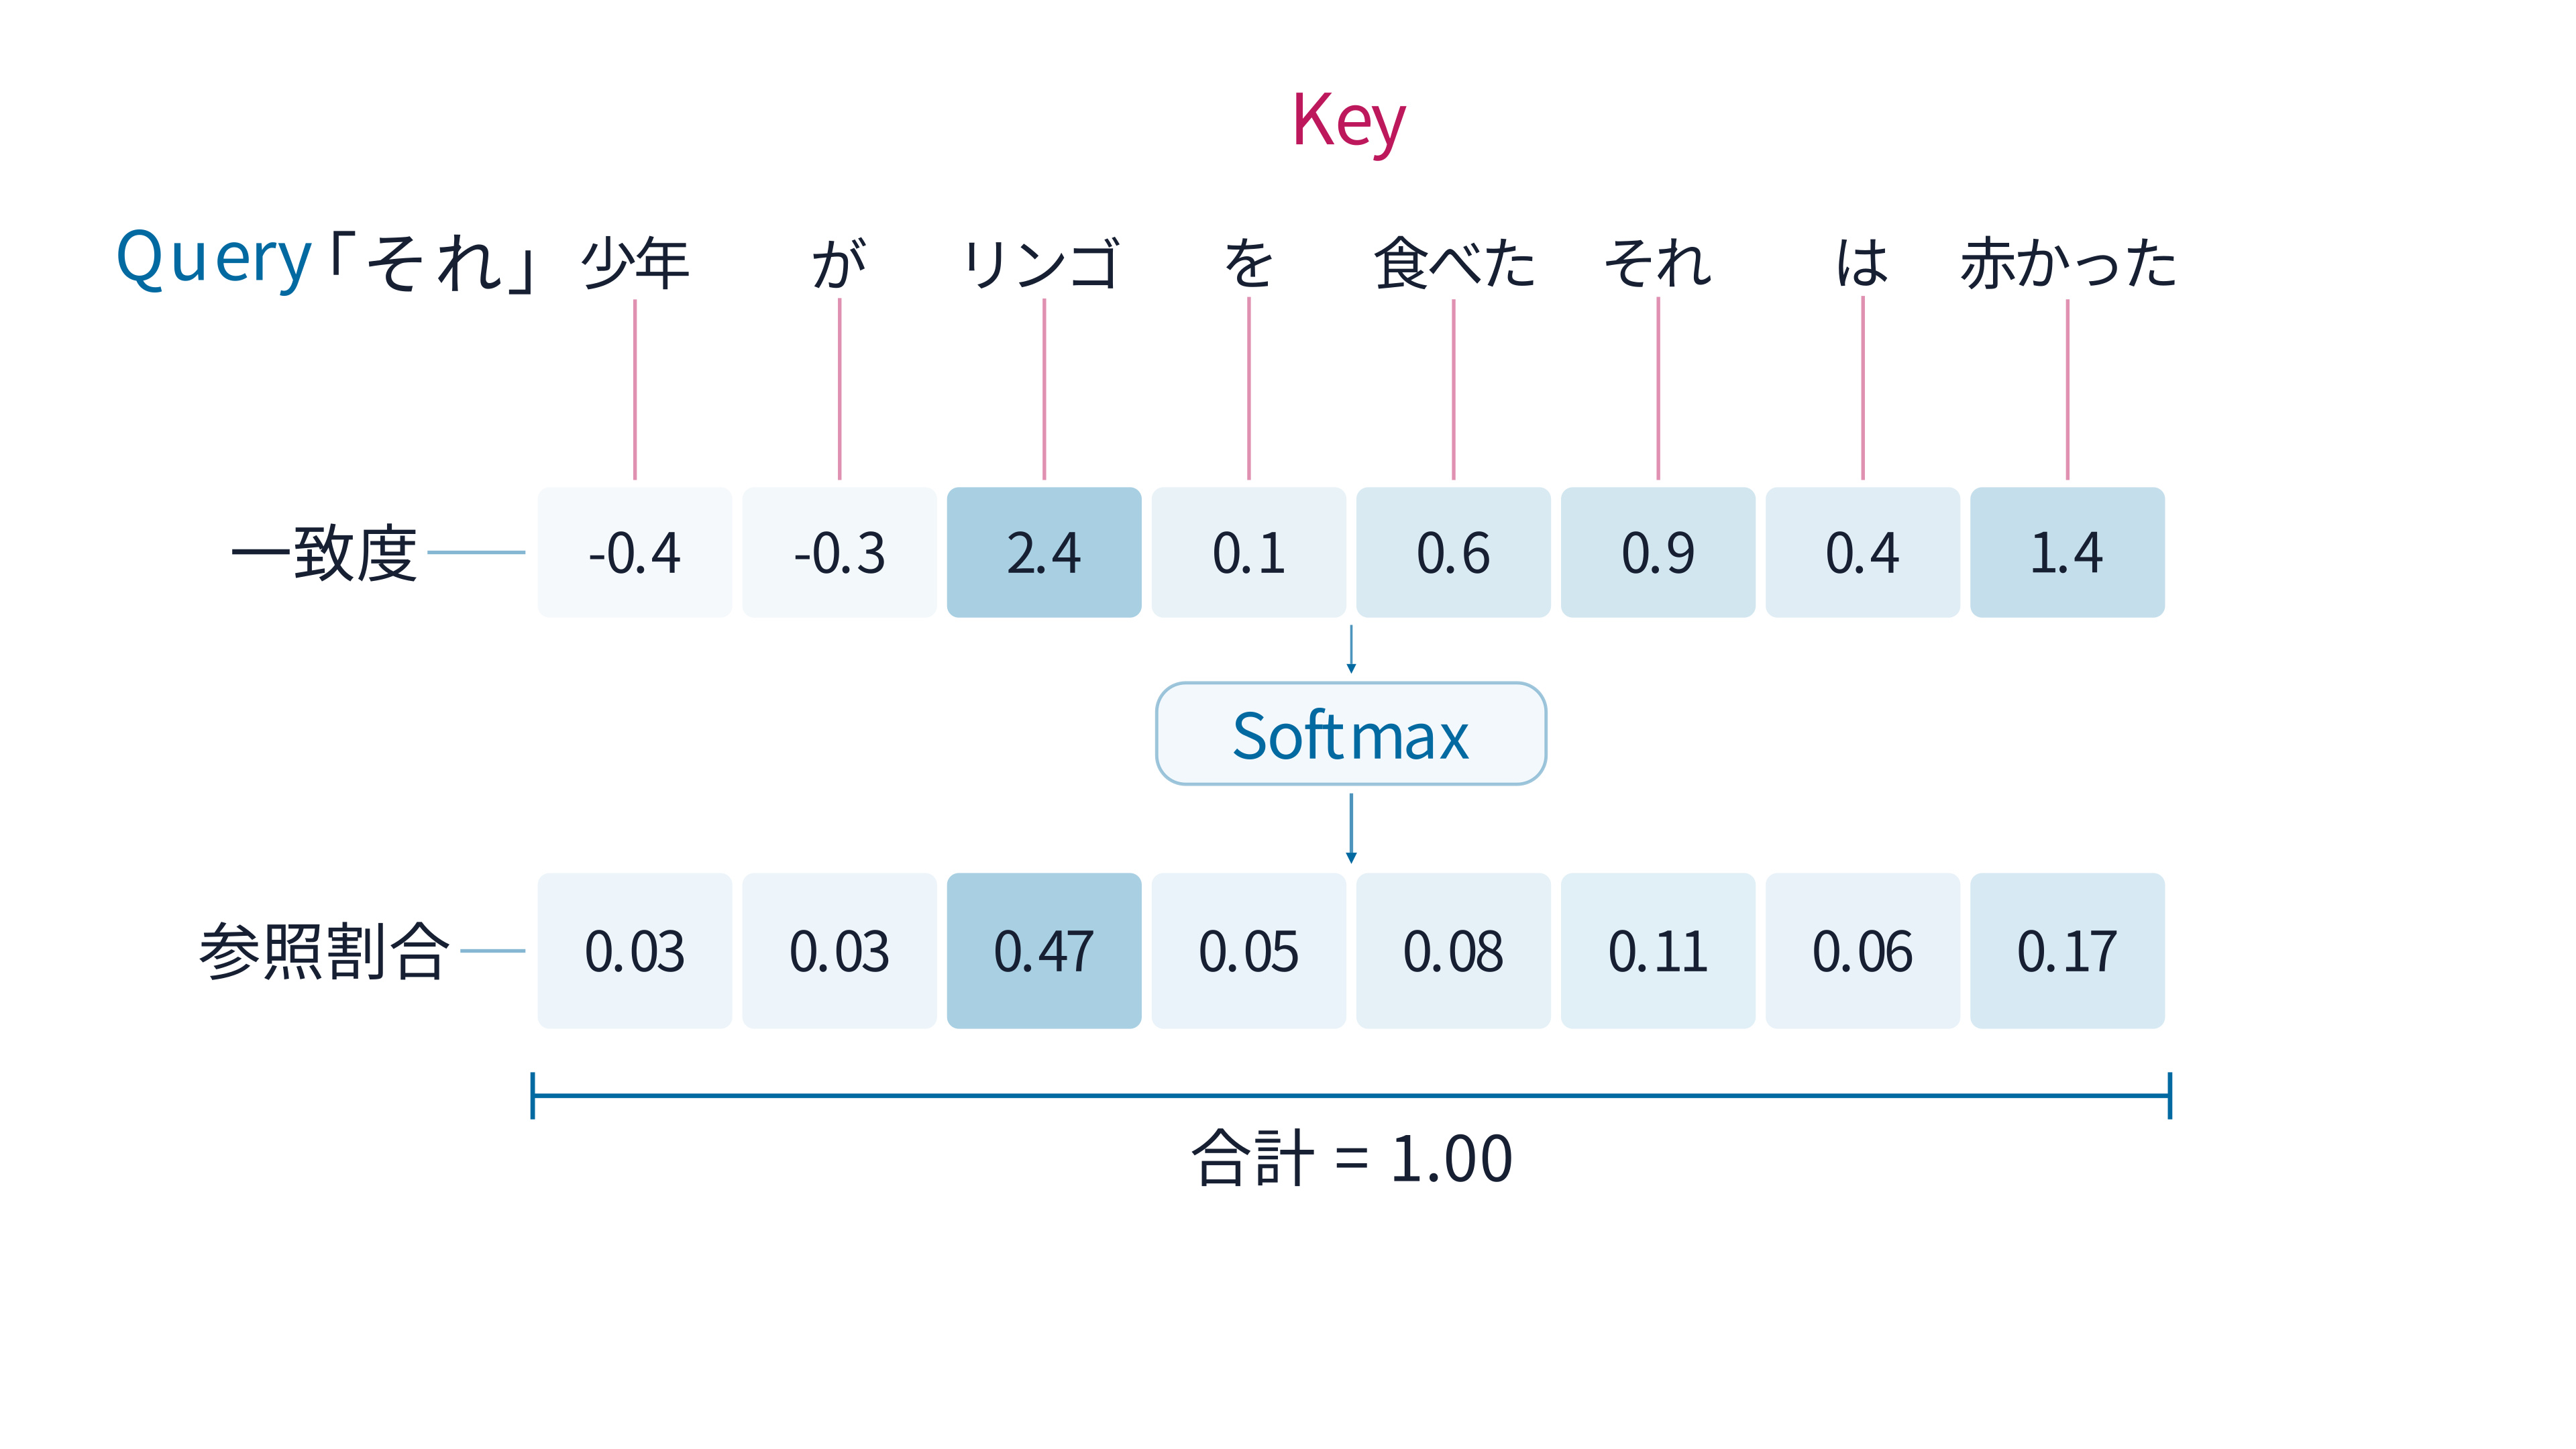
\includegraphics[width=\linewidth]{figures/fig07_softmax_reference_ratios.jpg}
  \caption{「それ」の参照割合}
  \label{fig:softmax-reference-ratios}
\end{figure}

\subsection{Valueを参照割合に応じて集める}
各入力のValueを参照割合に応じて足し合わせる。これにより、それぞれの入力は、関連するほかの入力から必要な情報を受け取る。
\begin{figure}[H]
  \centering
  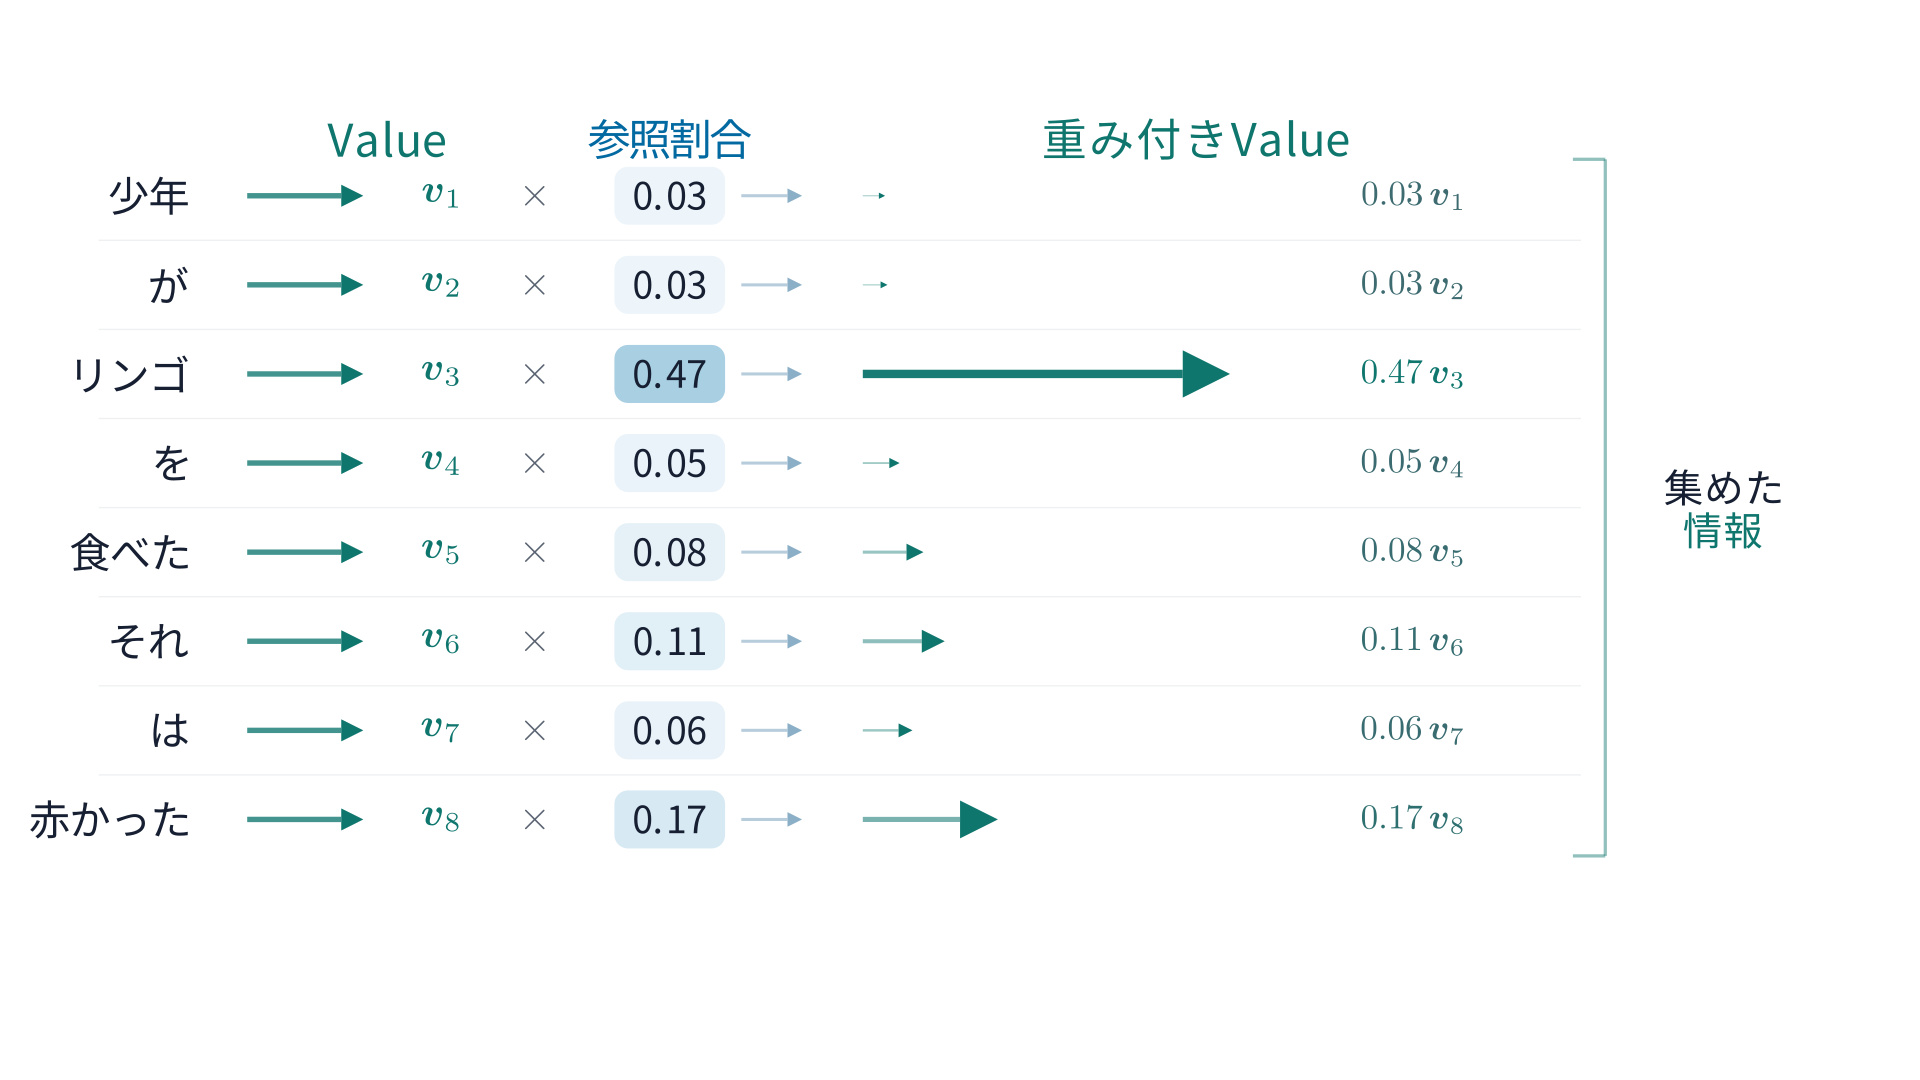
\includegraphics[width=\linewidth]{figures/fig08_weighted_value_collection.jpg}
  \caption{「それ」に集められる情報}
  \label{fig:weighted-value-collection}
\end{figure}

\subsection{詳細なアルゴリズム}
\begin{lstlisting}[caption=自己注意機構の詳細なアルゴリズム,label=lst:scaled_dot_product_attention]
Q = X @ W_Q
K = X @ W_K
V = X @ W_V

scores = Q @ K.T
scores = scores / sqrt(d_k)

attention_weights = softmax(scores, axis=-1)
outputs = attention_weights @ V
\end{lstlisting}


\section{まとめ}
本レポートでは、自己注意機構が複数の入力要素から必要な情報を選び、それぞれの要素へ反映する仕組みを説明した。自己注意機構は、入力からQuery、Key、Valueを作成し、QueryとKeyの一致度から各要素の参照割合を求め、その割合に応じてValueを集めることで新しい表現を生成する。

この処理により、各要素は周囲の要素との関係を考慮した情報を持つことができる。また、Query、Key、Valueを作る重み行列は学習によって更新されるため、モデルは学習データから「何を問い、何に答え、どの情報を伝えるべきか」を獲得する。つまり、自己注意機構における知識は重み行列の中に形成され、入力に応じた情報の参照と統合という形で利用される。

\end{document}
